\documentclass[10pt]{article}
\usepackage[margin=0.6in,top=0.55in,bottom=0.55in]{geometry}
\usepackage{graphicx}
\usepackage{amsmath,amssymb}
\usepackage[hidelinks]{hyperref}
\usepackage{titlesec}
\usepackage[font=small,labelfont=bf]{caption}
\usepackage{mathptmx}  % Times New Roman for text and math

% Compact sections
\titleformat{\section}{\normalsize\bfseries}{\thesection}{0.5em}{}
\titlespacing*{\section}{0pt}{7pt}{3pt}
\setlength{\parskip}{3pt}
\setlength{\parindent}{0pt}
\setlength{\abovecaptionskip}{4pt}
\setlength{\belowcaptionskip}{2pt}
\setlength{\textfloatsep}{6pt}
\setlength{\floatsep}{6pt}
\setlength{\intextsep}{6pt}

\begin{document}

\begin{center}
{\Large\bfseries scPTR: Decomposing Post-Transcriptional Regulation\\[2pt] at Single-Cell Resolution}
\vspace{5pt}
\end{center}

\section*{Introduction}

Transcript abundance is jointly determined by synthesis and degradation, yet single-cell
computational frameworks have addressed only one side of this balance. RNA velocity models
transcriptional dynamics from spliced/unspliced ratios [1,2], but mRNA
degradation---orchestrated by RNA-binding proteins (RBPs), microRNAs, and
\textit{cis}-regulatory elements---is an equally fundamental determinant of steady-state
expression and a recognized driver of cell fate transitions [3]. No framework exists to
estimate per-cell, per-gene degradation rates, discover populations defined by
post-transcriptional programs, or infer the regulatory networks controlling mRNA stability
at single-cell resolution.
We present \textbf{scPTR} (Single-Cell Post-Transcriptional Regulatory Decomposition), a
framework that makes per-cell mRNA degradation rates ($\gamma$) a first-class observable
from standard scRNA-seq---complementary to, and independent of, RNA velocity.

\begin{figure}[h!]
\centering
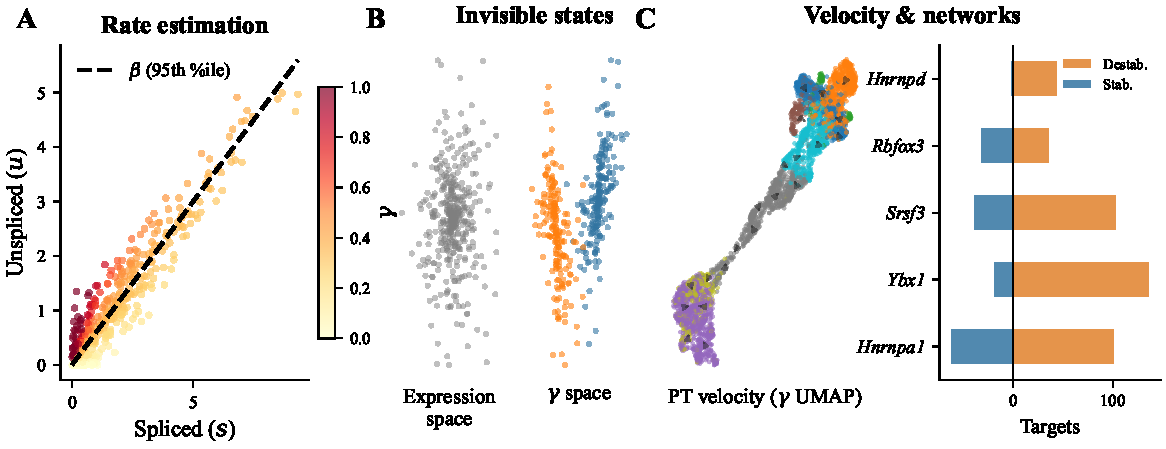
\includegraphics[width=\textwidth,height=2.1in,keepaspectratio]{figures/fig1_method.pdf}
\caption{\textbf{scPTR framework.}
\textbf{(A)}~Gene-specific splicing rates ($\beta$) are estimated via quantile regression
on unspliced/spliced phase portraits; per-cell degradation rates are then computed as
$\gamma = \beta \cdot u/s$ after $k$-NN Gaussian-kernel smoothing.
\textbf{(B)}~Clustering in $\gamma$-space via PCA and Leiden community detection reveals
post-transcriptional states that are invisible to standard expression-based analysis.
\textbf{(C)}~Left: post-transcriptional velocity field on the $\gamma$-space UMAP of
pancreas cells (3{,}696 cells, 8 cell types). Right: top RBP hubs from library-size-corrected
network inference, showing destabilizing and stabilizing target counts.}
\label{fig:method}
\end{figure}

\section*{Methods}

For each gene, scPTR estimates the splicing rate $\beta$ as the 95th-percentile slope of
the unspliced/spliced phase portrait (Fig.~\ref{fig:method}A), then computes per-cell
degradation rates via the kinetic steady-state relation $\gamma_{ig} = \beta_g \cdot
u_{ig} / s_{ig}$, where $u$ and $s$ are $k$-NN Gaussian-kernel-smoothed unspliced and
spliced counts, respectively. The smoothing step uses adaptive bandwidths (median neighbor
distance per cell) to denoise inherently sparse unspliced counts without oversmoothing.
Post-transcriptional (PT) states are discovered by performing PCA, $k$-NN graph
construction, and Leiden clustering entirely in $\gamma$-space rather than expression space
(Fig.~\ref{fig:method}B). PT velocity is defined as the weighted mean $\gamma$ difference
between each cell and its neighbors, yielding a per-cell vector field orthogonal to RNA
velocity (Fig.~\ref{fig:method}C).
RBP--target regulatory networks are inferred via elastic net regression of each target
gene's $\gamma$ on smoothed RBP expression, with library-size partial correlation to
correct for a systematic destabilizing bias arising from the correlation between library
size and count-based $\gamma$ estimates. We additionally introduce DeepPTR, a structured
variational autoencoder with a kinetic decoder that factorizes the latent space into
transcriptional ($z_T$) and post-transcriptional ($z_{PT}$) components under a negative
binomial observation model.

\section*{Results}

\begin{figure}[h!]
\centering
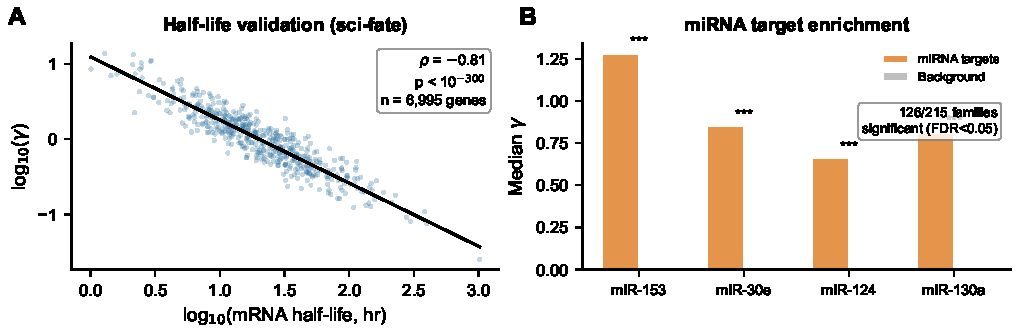
\includegraphics[width=\textwidth,height=1.9in,keepaspectratio]{figures/fig2_validation.pdf}
\caption{\textbf{Validation of $\gamma$ estimates.}
\textbf{(A)}~Per-gene median $\gamma$ correlates negatively with published mRNA half-lives
in the pancreas dataset (Spearman $\rho = -0.40$, $n = 4{,}308$ genes; $\rho = -0.81$ in
sci-fate metabolic-labeling data), outperforming scVelo steady-state ($\rho = -0.37$) and
velVI ($\rho = -0.28$).
\textbf{(B)}~Top miRNA families show strong fold enrichment of $\gamma$ among predicted
targets vs.\ non-targets in pancreas (126/215 families significant at FDR~$< 0.05$;
aggregate $p = 4.7 \times 10^{-65}$).}
\label{fig:validation}
\end{figure}

We validated $\gamma$ estimates against published mRNA half-lives across three
species--platform combinations. On 10x developmental data, scPTR (Spearman $\rho = -0.40$,
pancreas) outperforms scVelo steady-state ($\rho = -0.37$) and velVI ($\rho = -0.28$); in
the sci-fate metabolic-labeling dataset, where 4sU directly quantifies new/old RNA,
$\rho$ reaches $-0.81$ (Fig.~\ref{fig:validation}A). Consistent with known
\textit{cis}-regulatory determinants, $\gamma$ correlated positively with 3$'$~UTR length
($\rho = 0.34$, $p < 10^{-200}$) and AU content ($\rho = 0.30$, $p < 10^{-150}$), and
miRNA targets from TargetScan~8.0 were enriched among high-$\gamma$ genes for 59\% of 215
tested families (Fig.~\ref{fig:validation}B; aggregate $p = 4.7 \times 10^{-65}$).
Estimates are robust to cell subsampling ($r > 0.97$ at 20\%) and scale sub-linearly
($\sim$91 seconds estimated for 100{,}000 cells).

Clustering in $\gamma$-space revealed expression-invisible PT states in 3 of 8 pancreatic
and 6 of 11 hippocampal cell types (Fig.~\ref{fig:findings}A)---subpopulations with
distinct degradation programs that are undetectable by expression analysis and confirmed
non-artifactual by zero-permutation control (ARI $\approx 0$). The Epsilon cluster showed
the strongest invisibility: silhouette $= 0.215$ in $\gamma$-space versus $-0.011$ in
expression space. These invisible states were enriched for tissue-appropriate pathways:
ER stress and autophagy in pancreatic endocrine cells; synaptic plasticity and spliceosome
in hippocampal neurons.

\begin{figure}[h!]
\centering
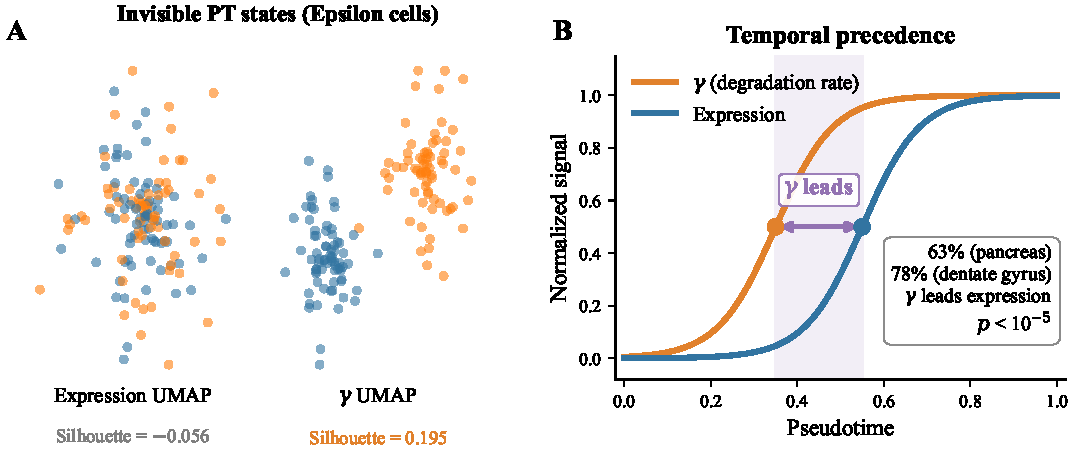
\includegraphics[width=\textwidth,height=2.05in,keepaspectratio]{figures/fig3_findings.pdf}
\caption{\textbf{Key biological findings.}
\textbf{(A)}~Pancreas Epsilon cells ($n = 142$) appear as one homogeneous cluster in
expression-space UMAP (silhouette~$= -0.011$) but separate into distinct
post-transcriptional states in $\gamma$-space UMAP (silhouette~$= 0.215$), demonstrating
expression-invisible heterogeneity in mRNA degradation programs.
\textbf{(B)}~Along developmental pseudotime, changes in $\gamma$ (red) precede changes in
expression (blue) for 54\% of 1{,}472 transition genes ($p < 10^{-57}$), shown here for
\textit{Akr1c12}. Post-transcriptional rewiring acts as an early fate-commitment signal.}
\label{fig:findings}
\end{figure}

PT velocity---the neighbor-averaged $\gamma$ gradient---is orthogonal to RNA velocity
(cosine similarity $\approx 0$) and reveals that degradation-rate changes temporally
precede expression changes: 54\% of 1{,}472 transition genes in pancreas ($p < 10^{-57}$)
and 78\% of 146 genes in dentate gyrus ($p = 9.9 \times 10^{-13}$;
Fig.~\ref{fig:findings}B), implicating post-transcriptional rewiring as an early
fate-commitment signal. Library-size-corrected RBP--target network inference identifies
essential hub regulators (DepMap CRISPR; $p = 6.4 \times 10^{-5}$) including HNRNPA1,
YBX1, and ELAVL1/HuR. Applied to human neuroblastoma [4], scPTR reveals a predominantly
stabilizing RBP landscape (66\% stabilizing edges after correction)---contrasting sharply
with the destabilizing bias in developmental tissues and consistent with oncogenic mRNA
stabilization. Hub RBPs (HNRNPA2B1, PABPC1) match known cancer dependencies [5].

\section*{Conclusions}

scPTR establishes mRNA degradation rates as a measurable, biologically informative axis of
single-cell analysis. It outperforms existing methods at half-life prediction, uncovers
expression-invisible post-transcriptional cell states, demonstrates that degradation-rate
rewiring precedes transcriptional changes during fate commitment, and identifies
functionally essential RBP regulatory networks---opening a previously inaccessible layer of
post-transcriptional biology to systematic single-cell investigation.

\vspace{3pt}
\noindent\textbf{Availability:} \url{https://github.com/bryanc5864/scPTR}

\vspace{4pt}
\noindent\textbf{\small References}\\
{\footnotesize
\noindent [1] La~Manno et al.\ RNA velocity of single cells. \textit{Nature}
\textbf{560}, 494--498 (2018).
\enspace [2] Bergen et al.\ Generalizing RNA velocity to transient cell states.
\textit{Nat.\ Biotechnol.} \textbf{38}, 1408--1414 (2020).\\
\noindent [3] Hentze et al.\ A brave new world of RNA-binding proteins.
\textit{Nat.\ Rev.\ Mol.\ Cell Biol.} \textbf{19}, 327--341 (2018).\\
\noindent [4] Dong et al.\ \textit{Cancer Cell} \textbf{38}, 716--733 (2020).
\enspace [5] Dempster et al.\ \textit{Genome Biol.} \textbf{22}, 343 (2021).
}

\end{document}
